\PassOptionsToPackage{unicode=true}{hyperref} % options for packages loaded elsewhere
\PassOptionsToPackage{hyphens}{url}
%
\documentclass[]{article}
\usepackage{lmodern}
\usepackage{amssymb,amsmath}
\usepackage{ifxetex,ifluatex}
\usepackage{fixltx2e} % provides \textsubscript
\ifnum 0\ifxetex 1\fi\ifluatex 1\fi=0 % if pdftex
  \usepackage[T1]{fontenc}
  \usepackage[utf8]{inputenc}
  \usepackage{textcomp} % provides euro and other symbols
\else % if luatex or xelatex
  \usepackage{unicode-math}
  \defaultfontfeatures{Ligatures=TeX,Scale=MatchLowercase}
\fi
% use upquote if available, for straight quotes in verbatim environments
\IfFileExists{upquote.sty}{\usepackage{upquote}}{}
% use microtype if available
\IfFileExists{microtype.sty}{%
\usepackage[]{microtype}
\UseMicrotypeSet[protrusion]{basicmath} % disable protrusion for tt fonts
}{}
\IfFileExists{parskip.sty}{%
\usepackage{parskip}
}{% else
\setlength{\parindent}{0pt}
\setlength{\parskip}{6pt plus 2pt minus 1pt}
}
\usepackage{hyperref}
\hypersetup{
            pdftitle={MLR Example},
            pdfauthor={SDS 291},
            pdfborder={0 0 0},
            breaklinks=true}
\urlstyle{same}  % don't use monospace font for urls
\usepackage[margin=1in]{geometry}
\usepackage{color}
\usepackage{fancyvrb}
\newcommand{\VerbBar}{|}
\newcommand{\VERB}{\Verb[commandchars=\\\{\}]}
\DefineVerbatimEnvironment{Highlighting}{Verbatim}{commandchars=\\\{\}}
% Add ',fontsize=\small' for more characters per line
\usepackage{framed}
\definecolor{shadecolor}{RGB}{248,248,248}
\newenvironment{Shaded}{\begin{snugshade}}{\end{snugshade}}
\newcommand{\AlertTok}[1]{\textcolor[rgb]{0.94,0.16,0.16}{#1}}
\newcommand{\AnnotationTok}[1]{\textcolor[rgb]{0.56,0.35,0.01}{\textbf{\textit{#1}}}}
\newcommand{\AttributeTok}[1]{\textcolor[rgb]{0.77,0.63,0.00}{#1}}
\newcommand{\BaseNTok}[1]{\textcolor[rgb]{0.00,0.00,0.81}{#1}}
\newcommand{\BuiltInTok}[1]{#1}
\newcommand{\CharTok}[1]{\textcolor[rgb]{0.31,0.60,0.02}{#1}}
\newcommand{\CommentTok}[1]{\textcolor[rgb]{0.56,0.35,0.01}{\textit{#1}}}
\newcommand{\CommentVarTok}[1]{\textcolor[rgb]{0.56,0.35,0.01}{\textbf{\textit{#1}}}}
\newcommand{\ConstantTok}[1]{\textcolor[rgb]{0.00,0.00,0.00}{#1}}
\newcommand{\ControlFlowTok}[1]{\textcolor[rgb]{0.13,0.29,0.53}{\textbf{#1}}}
\newcommand{\DataTypeTok}[1]{\textcolor[rgb]{0.13,0.29,0.53}{#1}}
\newcommand{\DecValTok}[1]{\textcolor[rgb]{0.00,0.00,0.81}{#1}}
\newcommand{\DocumentationTok}[1]{\textcolor[rgb]{0.56,0.35,0.01}{\textbf{\textit{#1}}}}
\newcommand{\ErrorTok}[1]{\textcolor[rgb]{0.64,0.00,0.00}{\textbf{#1}}}
\newcommand{\ExtensionTok}[1]{#1}
\newcommand{\FloatTok}[1]{\textcolor[rgb]{0.00,0.00,0.81}{#1}}
\newcommand{\FunctionTok}[1]{\textcolor[rgb]{0.00,0.00,0.00}{#1}}
\newcommand{\ImportTok}[1]{#1}
\newcommand{\InformationTok}[1]{\textcolor[rgb]{0.56,0.35,0.01}{\textbf{\textit{#1}}}}
\newcommand{\KeywordTok}[1]{\textcolor[rgb]{0.13,0.29,0.53}{\textbf{#1}}}
\newcommand{\NormalTok}[1]{#1}
\newcommand{\OperatorTok}[1]{\textcolor[rgb]{0.81,0.36,0.00}{\textbf{#1}}}
\newcommand{\OtherTok}[1]{\textcolor[rgb]{0.56,0.35,0.01}{#1}}
\newcommand{\PreprocessorTok}[1]{\textcolor[rgb]{0.56,0.35,0.01}{\textit{#1}}}
\newcommand{\RegionMarkerTok}[1]{#1}
\newcommand{\SpecialCharTok}[1]{\textcolor[rgb]{0.00,0.00,0.00}{#1}}
\newcommand{\SpecialStringTok}[1]{\textcolor[rgb]{0.31,0.60,0.02}{#1}}
\newcommand{\StringTok}[1]{\textcolor[rgb]{0.31,0.60,0.02}{#1}}
\newcommand{\VariableTok}[1]{\textcolor[rgb]{0.00,0.00,0.00}{#1}}
\newcommand{\VerbatimStringTok}[1]{\textcolor[rgb]{0.31,0.60,0.02}{#1}}
\newcommand{\WarningTok}[1]{\textcolor[rgb]{0.56,0.35,0.01}{\textbf{\textit{#1}}}}
\usepackage{graphicx,grffile}
\makeatletter
\def\maxwidth{\ifdim\Gin@nat@width>\linewidth\linewidth\else\Gin@nat@width\fi}
\def\maxheight{\ifdim\Gin@nat@height>\textheight\textheight\else\Gin@nat@height\fi}
\makeatother
% Scale images if necessary, so that they will not overflow the page
% margins by default, and it is still possible to overwrite the defaults
% using explicit options in \includegraphics[width, height, ...]{}
\setkeys{Gin}{width=\maxwidth,height=\maxheight,keepaspectratio}
\setlength{\emergencystretch}{3em}  % prevent overfull lines
\providecommand{\tightlist}{%
  \setlength{\itemsep}{0pt}\setlength{\parskip}{0pt}}
\setcounter{secnumdepth}{0}
% Redefines (sub)paragraphs to behave more like sections
\ifx\paragraph\undefined\else
\let\oldparagraph\paragraph
\renewcommand{\paragraph}[1]{\oldparagraph{#1}\mbox{}}
\fi
\ifx\subparagraph\undefined\else
\let\oldsubparagraph\subparagraph
\renewcommand{\subparagraph}[1]{\oldsubparagraph{#1}\mbox{}}
\fi

% set default figure placement to htbp
\makeatletter
\def\fps@figure{htbp}
\makeatother


\title{MLR Example}
\author{SDS 291}
\date{2/19/2020}

\begin{document}
\maketitle

We're using data from a sample of 104 homes in Northampton, MA to see
whether being close to the bike trail enhances the value of the home.
Specifically, we're looking at the association between square feet (a
house's size) and distance from the rail trail with the house's
estimated value in 2014. The variables we're using are:

\begin{itemize}
\tightlist
\item
  \texttt{Price2014}: Zillow price estimate from 2014 (in thousands of
  dollars)
\item
  \texttt{Distance}: Distance (in miles) to the nearest entry point to
  the rail trail network
\item
  \texttt{SquareFeet}: Square footage of interior finished space (in
  thousands of sf)
\end{itemize}

\hypertarget{regression-output}{%
\section{Regression Output}\label{regression-output}}

\begin{Shaded}
\begin{Highlighting}[]
\NormalTok{m1<-}\KeywordTok{lm}\NormalTok{(Price2014 }\OperatorTok{~}\StringTok{ }\NormalTok{SquareFeet }\OperatorTok{+}\StringTok{ }\NormalTok{Distance , }\DataTypeTok{data =}\NormalTok{ RailsTrails)}
\KeywordTok{summary}\NormalTok{(m1)}
\end{Highlighting}
\end{Shaded}

\begin{verbatim}
## 
## Call:
## lm(formula = Price2014 ~ SquareFeet + Distance, data = RailsTrails)
## 
## Residuals:
##     Min      1Q  Median      3Q     Max 
## -152.15  -30.27   -4.14   25.75  337.93 
## 
## Coefficients:
##             Estimate Std. Error t value Pr(>|t|)    
## (Intercept)   78.985     25.607   3.085  0.00263 ** 
## SquareFeet   147.920     12.765  11.588  < 2e-16 ***
## Distance     -15.788      7.586  -2.081  0.03994 *  
## ---
## Signif. codes:  0 '***' 0.001 '**' 0.01 '*' 0.05 '.' 0.1 ' ' 1
## 
## Residual standard error: 65.55 on 101 degrees of freedom
## Multiple R-squared:  0.6574, Adjusted R-squared:  0.6506 
## F-statistic: 96.89 on 2 and 101 DF,  p-value: < 2.2e-16
\end{verbatim}

\begin{enumerate}
\def\labelenumi{\arabic{enumi}.}
\tightlist
\item
  Write the fitted regression equation.
\end{enumerate}

\[\widehat{price} = \hat\beta_0 + \hat\beta_1 SquareFeet + \hat\beta_2 Distance\]
or

\[\widehat{price} = 78.985 + (147.920 \cdot SquareFeet) + (-15.788 \cdot Distance)\]
2. Test the hypothesis that distance from the rail trail has a linear
relationship with house price in 2014.

\(H_0: \beta = 0\)

\(H_A: \beta \ne 0\)

Since the t-statistic for the estimated relationship between distance
and price (t=-2.081) is larger (i.e., more negative) the critical value
\(t^*\) (\(t^*\)=-1.96), and the corresponding p-value (p=0.03994) is
below the 5\% level (i.e., p\textless{}0.05), we can reject the null
hypothesis and conclude that there is a significant linear relationship
between distance to the rail trail and price of a house, adjusted for
Square Feet.

\begin{enumerate}
\def\labelenumi{\arabic{enumi}.}
\setcounter{enumi}{2}
\tightlist
\item
  Calculate the 95\% confidence interval for Distance to 3 decimal
  places (t* = 1.96) and interpret in a sentence.
\end{enumerate}

\begin{Shaded}
\begin{Highlighting}[]
\NormalTok{lci<-(}\OperatorTok{-}\FloatTok{15.788}\OperatorTok{+}\NormalTok{(}\FloatTok{1.96}\OperatorTok{*}\FloatTok{7.586}\NormalTok{))}
\NormalTok{uci<-(}\OperatorTok{-}\FloatTok{15.788}\OperatorTok{-}\NormalTok{(}\FloatTok{1.96}\OperatorTok{*}\FloatTok{7.586}\NormalTok{))}
\KeywordTok{c}\NormalTok{(lci,uci)}
\end{Highlighting}
\end{Shaded}

\begin{verbatim}
## [1]  -0.91944 -30.65656
\end{verbatim}

We are 95\% confident that the true relationship between distance and
house price is between \$919.44 and \$30,656.56 lower home price for
each 1 mile distance further away from the rail trail, adjusted for
house size.

\begin{enumerate}
\def\labelenumi{\arabic{enumi}.}
\setcounter{enumi}{3}
\tightlist
\item
  What price would this model predict for a 1700 square foot house that
  it .986 miles from the rail trail? (Be cautious with the units)
\end{enumerate}

\begin{Shaded}
\begin{Highlighting}[]
\NormalTok{predicted<-(}\FloatTok{78.985} \OperatorTok{+}\StringTok{ }\NormalTok{(}\FloatTok{147.920}\OperatorTok{*}\FloatTok{1.7}\NormalTok{) }\OperatorTok{+}\StringTok{ }\NormalTok{(}\OperatorTok{-}\FloatTok{15.788}\OperatorTok{*}\FloatTok{0.96}\NormalTok{) )}
\NormalTok{predicted}
\end{Highlighting}
\end{Shaded}

\begin{verbatim}
## [1] 315.2925
\end{verbatim}

The model would predict a house with 1700 square feet that is 0.986
miles from the rail trail would have a value of \$315,292.50.

\begin{enumerate}
\def\labelenumi{\arabic{enumi}.}
\setcounter{enumi}{3}
\tightlist
\item
  An actual house in this dataset that is 1700 square feet and .986
  miles from the rail trail entrance had an Zillow price estimate of
  \$222,864. Calculate the residual for this house and interpret it in a
  sentence in the context of this problem.
\end{enumerate}

\begin{Shaded}
\begin{Highlighting}[]
\NormalTok{actual<-}\FloatTok{222.864}
\NormalTok{actual }\OperatorTok{-}\StringTok{ }\NormalTok{predicted}
\end{Highlighting}
\end{Shaded}

\begin{verbatim}
## [1] -92.42852
\end{verbatim}

The residual for this particular home was \$-92,428.52 meaning the house
had lower \emph{actual} price than the mdoel would have expected by
\$92,482.52. In other words, the model overestimtated the price of this
particular house.

\newpage

\hypertarget{residuals-and-model-error}{%
\section{Residuals and Model Error}\label{residuals-and-model-error}}

\begin{Shaded}
\begin{Highlighting}[]
\KeywordTok{anova}\NormalTok{(m1)}
\end{Highlighting}
\end{Shaded}

\begin{verbatim}
## Analysis of Variance Table
## 
## Response: Price2014
##             Df Sum Sq Mean Sq  F value  Pr(>F)    
## SquareFeet   1 813976  813976 189.4454 < 2e-16 ***
## Distance     1  18611   18611   4.3316 0.03994 *  
## Residuals  101 433959    4297                     
## ---
## Signif. codes:  0 '***' 0.001 '**' 0.01 '*' 0.05 '.' 0.1 ' ' 1
\end{verbatim}

\begin{enumerate}
\def\labelenumi{\arabic{enumi}.}
\tightlist
\item
  Calculate the \(R^2\) (same equation as simple linear regression,
  p.103-104) and Adjusted \(R^2\) for the model (see p.105 for the
  equation). Interpret each in a sentence.
\end{enumerate}

\[ R^2 = 1 - \frac{SSError}{SSTotal} \] and

\[ AdjR^2 = 1 - \frac{\frac{SSError}{n-k-1}}{\frac{SSTotal}{n-1}} \]

\begin{Shaded}
\begin{Highlighting}[]
\NormalTok{SSE<-}\StringTok{ }\DecValTok{433959}
\NormalTok{SST<-}\StringTok{ }\DecValTok{813976}\OperatorTok{+}\DecValTok{18611}\OperatorTok{+}\DecValTok{433959}
\NormalTok{SSM<-}\StringTok{ }\DecValTok{813976}\OperatorTok{+}\DecValTok{18611}

\NormalTok{RSq<-}\StringTok{ }\DecValTok{1}\OperatorTok{-}\StringTok{ }\NormalTok{(SSE}\OperatorTok{/}\NormalTok{SST)}
\NormalTok{RSq}
\end{Highlighting}
\end{Shaded}

\begin{verbatim}
## [1] 0.6573681
\end{verbatim}

\begin{Shaded}
\begin{Highlighting}[]
\NormalTok{n<-}\StringTok{ }\KeywordTok{nrow}\NormalTok{(RailsTrails)}
\NormalTok{k<-}\DecValTok{2}
\NormalTok{AdjRSq<-}\StringTok{ }\DecValTok{1}\OperatorTok{-}\StringTok{ }\NormalTok{( (SSE }\OperatorTok{/}\StringTok{ }\NormalTok{(n}\OperatorTok{-}\NormalTok{k}\DecValTok{-1}\NormalTok{)) }\OperatorTok{/}\StringTok{ }\NormalTok{( SST }\OperatorTok{/}\StringTok{ }\NormalTok{(n}\DecValTok{-1}\NormalTok{)) )}
\NormalTok{AdjRSq}
\end{Highlighting}
\end{Shaded}

\begin{verbatim}
## [1] 0.6505834
\end{verbatim}

65.74\% of the variation in house prices explained by the model, as
reflected by \(R^2\). Adjusted \(R^2\) takes into account how many
explanatory variables there are in the model, and its value suggests
that 65.05\% of the variation in house prices is explained by this
model. Adjusted \(R^2\) is useful for comparing across models,
especially as the number of explanatory variables change between models,
and is the better measure to use in multiple regression.

\begin{enumerate}
\def\labelenumi{\arabic{enumi}.}
\tightlist
\item
  Calculate the regression standard error for this model (p.99) and
  interepret it in a sentence.
\end{enumerate}

\begin{Shaded}
\begin{Highlighting}[]
\KeywordTok{library}\NormalTok{(broom)}
\NormalTok{m1_data<-}\KeywordTok{augment}\NormalTok{(m1)}

\NormalTok{SSE <-}\StringTok{ }\KeywordTok{sum}\NormalTok{((m1_data}\OperatorTok{$}\NormalTok{.resid)}\OperatorTok{^}\DecValTok{2}\NormalTok{)}
\NormalTok{SSE}
\end{Highlighting}
\end{Shaded}

\begin{verbatim}
## [1] 433959.5
\end{verbatim}

\begin{Shaded}
\begin{Highlighting}[]
\NormalTok{RSE<-}\KeywordTok{sqrt}\NormalTok{(SSE}\OperatorTok{/}\NormalTok{(n}\OperatorTok{-}\NormalTok{k}\DecValTok{-1}\NormalTok{))}
\NormalTok{RSE}
\end{Highlighting}
\end{Shaded}

\begin{verbatim}
## [1] 65.54867
\end{verbatim}

The average amount of error in the model is 65.55; in other words, the
model's estimates of a home's price is off by \$65,548.67.

\begin{enumerate}
\def\labelenumi{\arabic{enumi}.}
\tightlist
\item
  Calculate the F statistic for the model:
  \(F = \frac{MSModel}{MSError}\) (see p.102 for making sense of the
  ANOVA table)
\end{enumerate}

\begin{Shaded}
\begin{Highlighting}[]
\NormalTok{MSM<-SSM}\OperatorTok{/}\NormalTok{k}
\NormalTok{MSE<-SSE}\OperatorTok{/}\NormalTok{(n}\OperatorTok{-}\NormalTok{k}\DecValTok{-1}\NormalTok{)}
\NormalTok{FStat<-MSM}\OperatorTok{/}\NormalTok{MSE}
\NormalTok{FStat}
\end{Highlighting}
\end{Shaded}

\begin{verbatim}
## [1] 96.88841
\end{verbatim}

\begin{enumerate}
\def\labelenumi{\arabic{enumi}.}
\tightlist
\item
  State the null and alternative hypotheses for the F test (see p.102).
  Look at the F Distribution calculator (at
  \url{https://gallery.shinyapps.io/dist_calc/}) and estimate the
  p-value for your F statistic with the degrees of freedom above (it
  will be an approximation - the slider bars won't go as high as you
  need them to - but it gives you the rough answer for your hypothesis).
  What do you conclude about your hypothesis?
\end{enumerate}

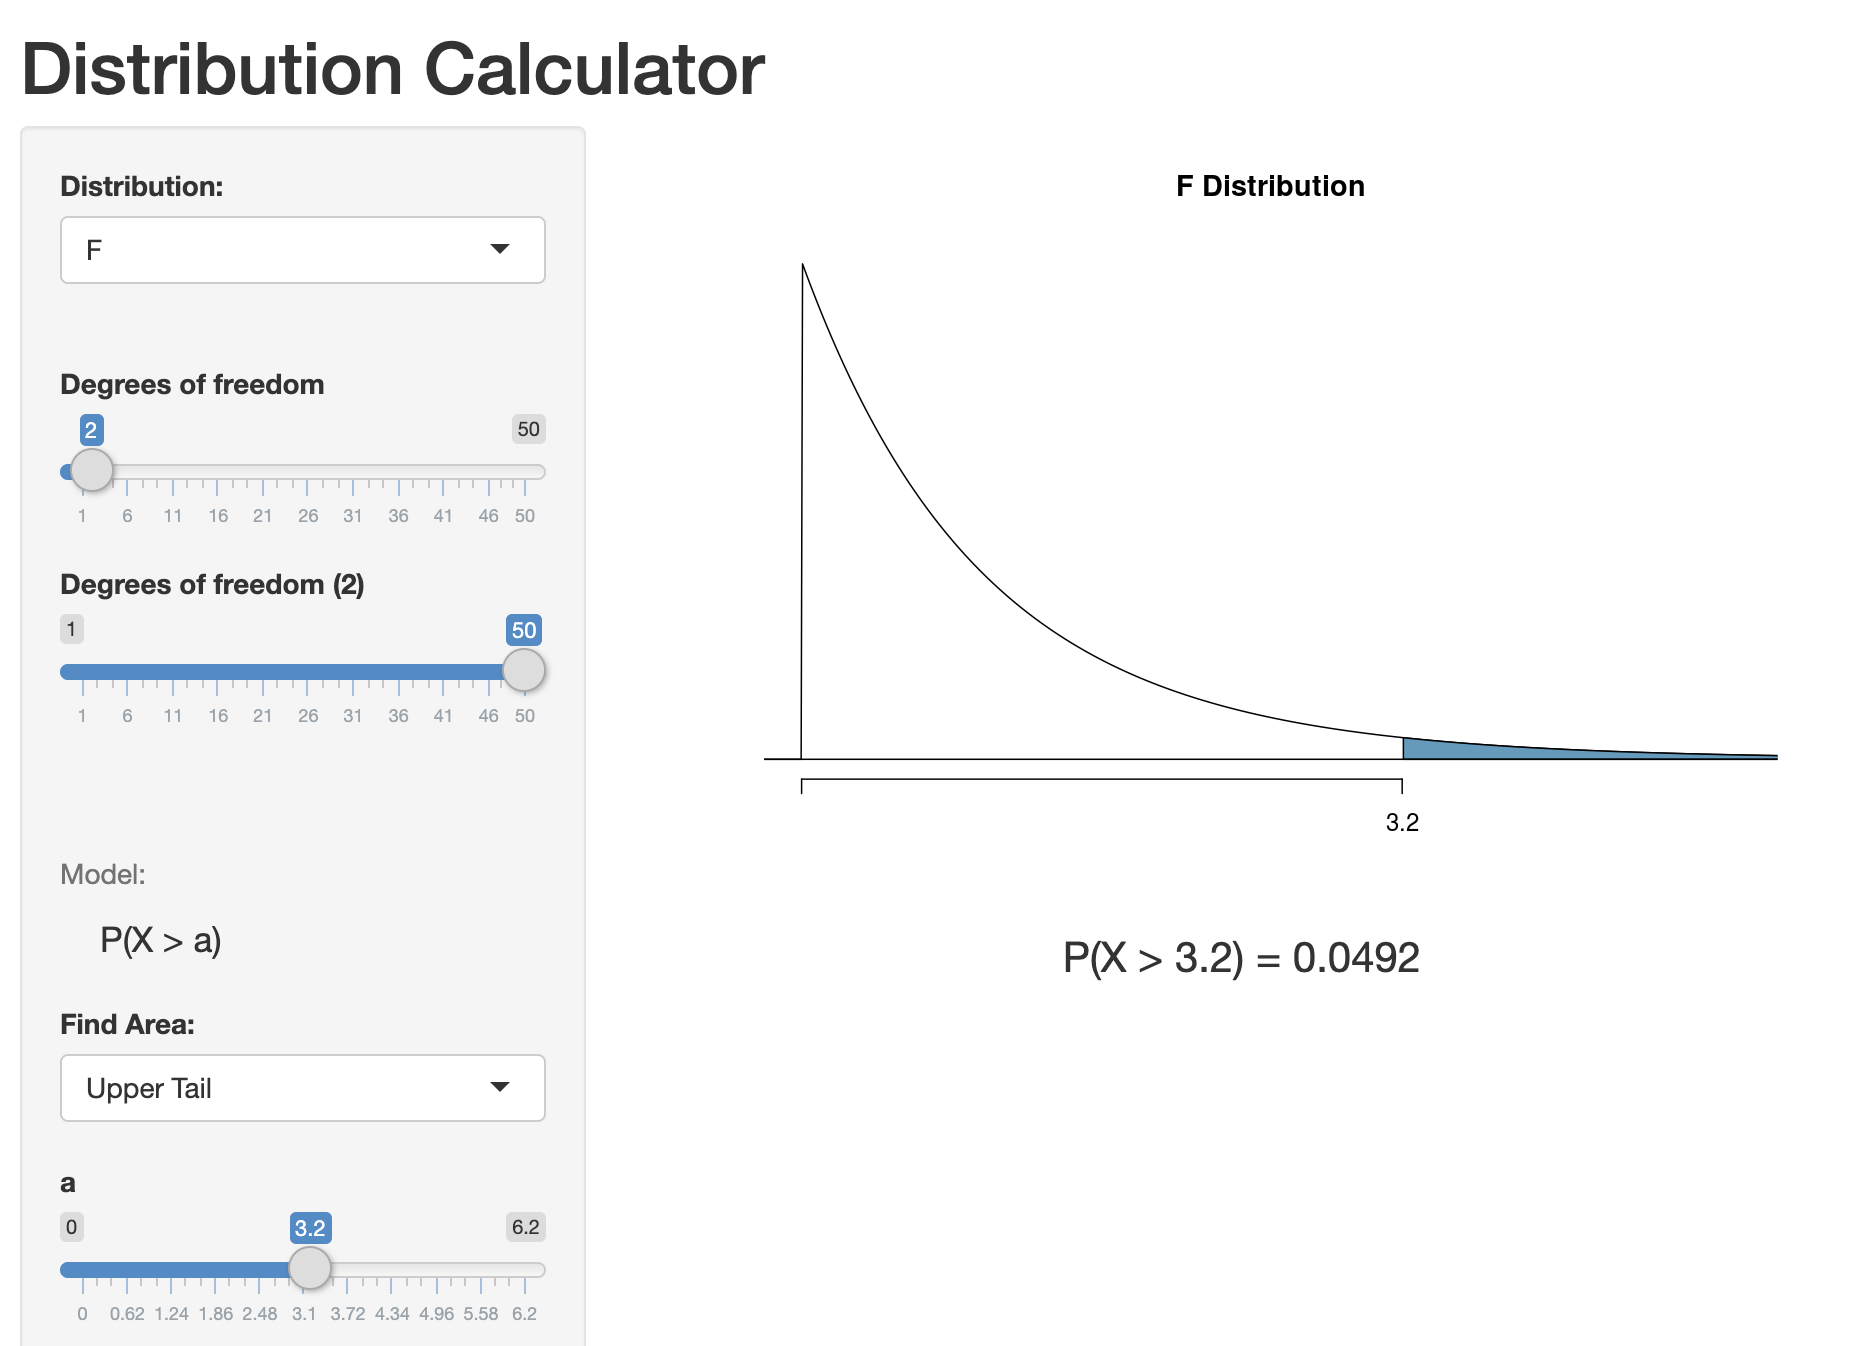
\includegraphics{FStatistic.png}

\(H_0: \beta_1=\beta_2=0\)

\(H_A: \beta_1=\beta_2 \ne 0\)

Given that our FStatistic (96.88) is much larger than the critical value
of 3.2, the pvalue should be much smaller than 0.05. From the summary
output we see that an F(2,102)=96.88, p\textless{}0.001. Thus, we could
reject the null hypothesis that the model (\(\hat\beta_1\) and
\(\hat\beta_2\)) explains none of the variation in the house prices and
conclude that the model overall does explain a significant amount of
variation in house prices.

\end{document}
